\section{Übung 4 – Abtastung und Quantisierung}

\subsection*{Grundprinzip}

Um ein wert- und zeitkontinuierliches Signal zu digitalisieren, wird es in zwei Schritten 
verarbeitet:

\begin{enumerate}
    \item \textbf{Abtastung:} Das Signal wird in gleichmäßigen Zeitabständen $T_A$ abgetastet.
          Ergebnis: wertkontinuierliches, zeitdiskretes Signal $x[n] = x(n \cdot T_A)$.
    \item \textbf{Quantisierung:} Die Abtastwerte werden einer von $N$ diskreten Stufen zugeordnet.
          Ergebnis: vollständig diskretes Signal $\hat{x}[n]$.
\end{enumerate}

\begin{figure}[H]
\centering
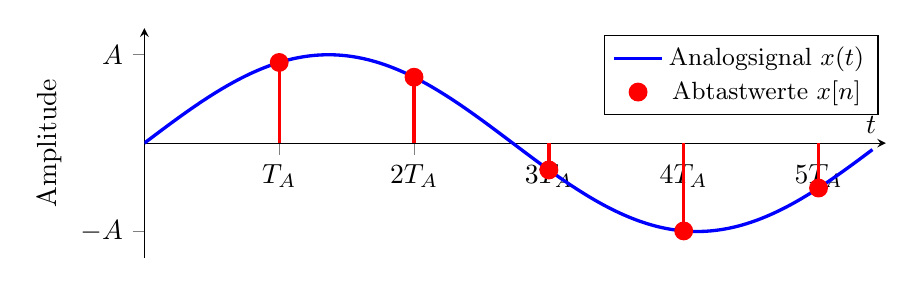
\begin{tikzpicture}
\begin{axis}[
    width=11cm, height=4.5cm,
    xlabel={$t$},
    ylabel={Amplitude},
    xmin=0, xmax=5.5,
    ymin=-1.3, ymax=1.3,
    axis x line=middle,
    axis y line=left,
    xtick={1,2,3,4,5},
    xticklabels={$T_A$, $2T_A$, $3T_A$, $4T_A$, $5T_A$},
    ytick={-1, 1},
    yticklabels={$-A$, $A$},
    tick align=outside,
    legend style={at={(0.99,0.97)}, anchor=north east, font=\small},
    every axis plot/.append style={line width=1.2pt},
]
\addplot[blue, smooth, domain=0:5.4, samples=200] {sin(deg(x*1.15))};
\addlegendentry{Analogsignal $x(t)$}
\addplot[red, ycomb, mark=*, mark size=2.8pt, mark options={fill=red}]
    coordinates {
        (1, {sin(deg(1.15))})
        (2, {sin(deg(2.30))})
        (3, {sin(deg(3.45))})
        (4, {sin(deg(4.60))})
        (5, {sin(deg(5.75))})
    };
\addlegendentry{Abtastwerte $x[n]$}
\end{axis}
\end{tikzpicture}
\caption{Abtastung: Aus dem kontinuierlichen Signal (blau) werden in Abständen $T_A$ Werte 
    entnommen (rot).}
\end{figure}

\subsection*{Beispiel: Abtastperiode und Stufenbreite}

Gegeben sei die Abtastfrequenz $f_A = 10\,\text{kHz}$, wobei $\text{Hz} = \text{s}^{-1}$.
Die Abtastperiode beträgt:

$$
T_A = \frac{1}{f_A} = \frac{1}{10\,000\,\text{s}^{-1}} = 0{,}1\,\text{ms}
$$

Für den Wertebereich $[-0{,}4,\; 0{,}4]$ (Gesamtbreite $x_{\max} - x_{\min} = 0{,}8$)
und eine Stufenbreite $\delta x = 0{,}2$ ergibt sich die Stufenanzahl:

$$
N = \frac{x_{\max} - x_{\min}}{\delta x} = \frac{0{,}8}{0{,}2} = 4,
\qquad
\delta x = \frac{0{,}8}{N} = \frac{0{,}8}{4} = 0{,}2
$$

Der Rekonstruktionswert der untersten Stufe ergibt sich als Mittelpunkt des ersten Intervalls:

$$
x_1 = \frac{-0{,}4 + (-0{,}2)}{2} = -0{,}3
$$

\subsection*{Midrise-Kennlinie}

Die \textbf{Midrise-Kennlinie} ist eine Treppenfunktion, bei der die steigende Flanke durch den
Ursprung $(0,\,0)$ verläuft. Beim \textbf{Midtread-Quantisierer} liegt im Ursprung hingegen
eine konstante Stufe – die Kurve verläuft dort flach.

\begin{figure}[H]
\centering
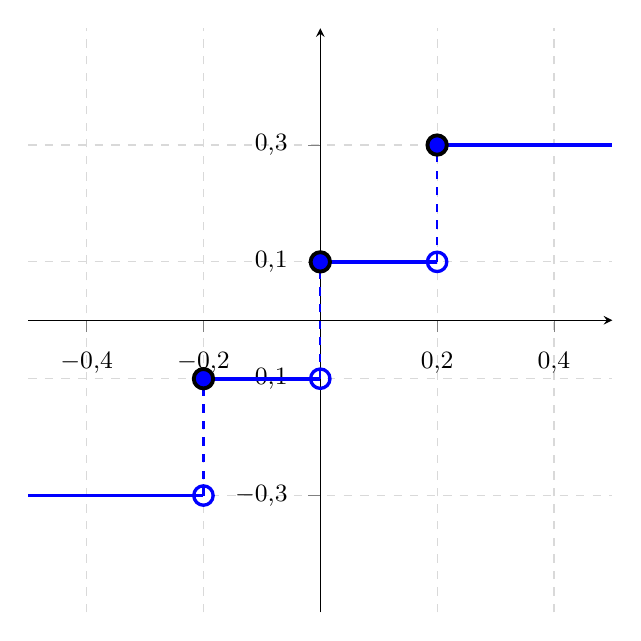
\begin{tikzpicture}
\begin{axis}[
    width=9cm, height=9cm,
    xmin=-0.50, xmax=0.50,
    ymin=-0.50, ymax=0.50,
    axis lines=center,
    xtick={-0.4,-0.2,0.2,0.4},
    xticklabels={$-0{,}4$, $-0{,}2$, $0{,}2$, $0{,}4$},
    ytick={-0.3,-0.1,0.1,0.3},
    yticklabels={$-0{,}3$, $-0{,}1$, $0{,}1$, $0{,}3$},
    x tick label style={anchor=north, yshift=-4pt, font=\small},
    y tick label style={anchor=east, xshift=-4pt, font=\small},
    grid=both,
    grid style={dashed, gray!30},
    tick align=outside,
    every axis plot/.append style={line width=1.4pt},
]
% Horizontale Stufen
\addplot[blue] coordinates {(-0.50,-0.3) (-0.20,-0.3)};
\addplot[blue] coordinates {(-0.20,-0.1) ( 0.00,-0.1)};
\addplot[blue] coordinates {( 0.00, 0.1) ( 0.20, 0.1)};
\addplot[blue] coordinates {( 0.20, 0.3) ( 0.50, 0.3)};
% Gestrichelte Übergänge
\addplot[blue, dashed, line width=0.8pt] coordinates {(-0.2,-0.3) (-0.2,-0.1)};
\addplot[blue, dashed, line width=0.8pt] coordinates {( 0.0,-0.1) ( 0.0, 0.1)};
\addplot[blue, dashed, line width=0.8pt] coordinates {( 0.2, 0.1) ( 0.2, 0.3)};
% Offene Kreise (nicht inbegriffen)
\addplot[only marks, mark=o, mark size=3.5pt,
         mark options={draw=blue, fill=white, line width=1.2pt}]
    coordinates {(-0.2,-0.3) (0.0,-0.1) (0.2,0.1)};
% Gefüllte Kreise (inbegriffen)
\addplot[only marks, mark=*, mark size=3.5pt, mark options={fill=blue}]
    coordinates {(-0.2,-0.1) (0.0,0.1) (0.2,0.3)};
\end{axis}
\end{tikzpicture}
\caption{Midrise-Kennlinie: $N = 4$ Stufen, $\delta x = 0{,}2$, Wertebereich $[-0{,}4,\,0{,}4]$.
Die Treppenfunktion steigt am Ursprung und erfüllt $Q(x) \neq 0$ für alle $x \neq 0$.}
\end{figure}

Für das Beispiel ($N = 4$, $\delta x = 0{,}2$, Midrise) ergeben sich folgende
Quantisierungsintervalle und Rekonstruktionswerte $\hat{x}$:

\begin{itemize}
    \item $x \in [{-0{,}4},\; {-0{,}2})$ \quad$\Rightarrow$\quad $\hat{x} = {-0{,}3}$
    \item $x \in [{-0{,}2},\; 0)$         \quad$\Rightarrow$\quad $\hat{x} = {-0{,}1}$
    \item $x \in [0,\; 0{,}2)$            \quad$\Rightarrow$\quad $\hat{x} = 0{,}1$
    \item $x \in [0{,}2,\; 0{,}4]$        \quad$\Rightarrow$\quad $\hat{x} = 0{,}3$
\end{itemize}

\begin{figure}[H]
\centering
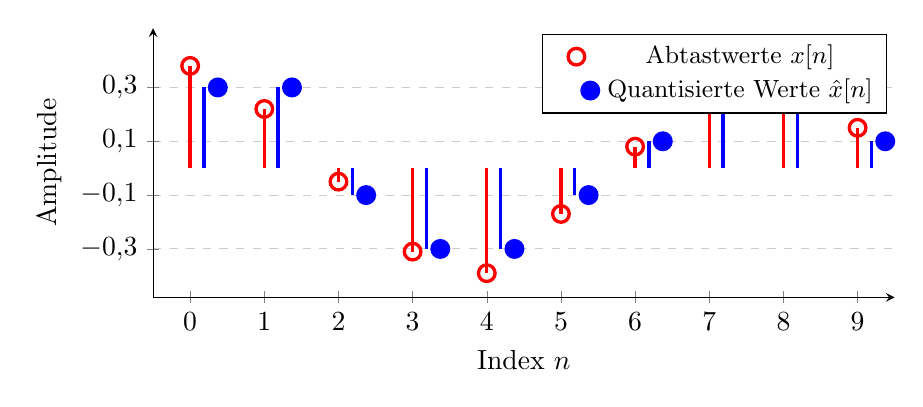
\begin{tikzpicture}
\begin{axis}[
    width=11cm, height=5cm,
    xlabel={Index $n$},
    ylabel={Amplitude},
    xmin=-0.5, xmax=9.5,
    ymin=-0.48, ymax=0.52,
    axis lines=left,
    xtick={0,1,...,9},
    ytick={-0.3,-0.1,0.1,0.3},
    yticklabels={$-0{,}3$, $-0{,}1$, $0{,}1$, $0{,}3$},
    ymajorgrids=true,
    grid style={dashed, gray!40},
    legend style={at={(0.99,0.98)}, anchor=north east, font=\small},
    every axis plot/.append style={line width=1.2pt},
]
% Originale Abtastwerte
\addplot[red, ycomb, mark=o, mark size=3pt,
         mark options={draw=red, fill=white, line width=1.2pt}]
    coordinates {
        (0,  0.38) (1,  0.22) (2, -0.05) (3, -0.31) (4, -0.39)
        (5, -0.17) (6,  0.08) (7,  0.28) (8,  0.39) (9,  0.15)
    };
\addlegendentry{Abtastwerte $x[n]$}
% Quantisierte Werte (leicht versetzt zur besseren Lesbarkeit)
\addplot[blue, ycomb, mark=*, mark size=3pt, mark options={fill=blue},
         transform canvas={xshift=5pt}]
    coordinates {
        (0,  0.3) (1,  0.3) (2, -0.1) (3, -0.3) (4, -0.3)
        (5, -0.1) (6,  0.1) (7,  0.3) (8,  0.3) (9,  0.1)
    };
\addlegendentry{Quantisierte Werte $\hat{x}[n]$}
\end{axis}
\end{tikzpicture}
\caption{Quantisierung: Die Abtastwerte (rot) werden den nächstgelegenen Quantisierungsstufen
(blau, gestrichelte Linien) zugeordnet. Jede Stufe entspricht dem Rekonstruktionswert $\hat{x}$.}
\end{figure}

Nach der Quantisierung aller Abtastwerte entsteht aus dem ursprünglich kontinuierlichen Signal
ein vollständig diskretes, digitales Signal.




% -------------------------------------------------- %
%                    Tutorium 4                      %
% -------------------------------------------------- %

\subsection{Tutorium 4}

\subsubsection*{Motivation: Warum abtasten und quantisieren?}

Digitale Systeme können nur mit endlich vielen, diskreten Werten umgehen. Um ein physikalisches
Signal – das in der Natur wert- und zeitkontinuierlich vorliegt – digital verarbeiten zu können,
sind zwei Schritte nötig:

\begin{enumerate}
    \item \textbf{Abtastung} (zeitdiskret machen): Das Signal wird nur zu Zeitpunkten $n \cdot T_A$
          ausgewertet. Ergebnis: wertkontinuierliches, zeitdiskretes Signal $x[n]$.
    \item \textbf{Quantisierung} (wertdiskret machen): Die Abtastwerte werden auf $N$ diskrete
          Stufen abgebildet. Ergebnis: vollständig diskretes Signal $\hat{x}[n]$.
\end{enumerate}

\subsubsection*{Midrise vs.\ Midtread}

Beide Quantisierungskennlinien ordnen jedem Eingangswert $x$ einen diskreten Rekonstruktionswert
$\hat{x}$ zu, unterscheiden sich aber im Verhalten am Ursprung:

\begin{itemize}
    \item \textbf{Midrise:} Die Stufengrenze liegt genau bei $x = 0$. Es gibt keine eigene Stufe
          für den Nullpunkt – die Kennlinie steigt dort durch. Sinnvoll bei gleichmäßig verteilten
          Signalen mit gerader Stufenanzahl $N$.
    \item \textbf{Midtread:} Die Stufe liegt mittig über $x = 0$, d.\,h.\ $Q(0) = 0$. Vorteil:
          Schwache Signale nahe Null werden exakt auf $0$ quantisiert – kein Rauschen bei Stille.
          Sinnvoll bei Signalen, die häufig um die Null schwingen.
\end{itemize}

\subsubsection*{Rekonstruktion durch Interpolation}

Um das zeitdiskrete Signal $x[n]$ wieder in ein zeitkontinuierliches Signal $x(t)$ umzuwandeln,
werden gewichtete Basisfunktionen $g_k(t)$ übereinandergelegt:

$$
x(t) = \sum_{k=-\infty}^{\infty} x[k] \cdot g_k(t)
$$

Die Wahl der Basisfunktion $g_k(t)$ bestimmt Qualität und Glattheitsgrad der Rekonstruktion:

\begin{itemize}
    \item \textbf{0.\,Ordnung – Zero-Order Hold (ZOH):} $g_k(t)$ ist ein Rechteckimpuls. Der
          Abtastwert wird bis zum nächsten Zeitpunkt konstant gehalten. Ergebnis: zeitkontinuierlich,
          aber wertdiskret (Treppenfunktion).
    \item \textbf{1.\,Ordnung – Lineare Interpolation:} $g_k(t)$ ist ein Dreieckimpuls. Benachbarte
          Abtastwerte werden linear verbunden. Ergebnis: zeitkontinuierlich und stetig,
          aber nicht differenzierbar (Knicke an den Abtastzeitpunkten).
    \item \textbf{Ideale Interpolation – $\operatorname{si}$-Funktion:} Mit
          $g_k(t) = \operatorname{si}\!\left(\tfrac{t - k T_A}{T_A}\right)$ wird bei Einhaltung
          des Nyquist-Kriteriums das Originalsignal exakt rekonstruiert.
\end{itemize}

\begin{figure}[H]
\centering
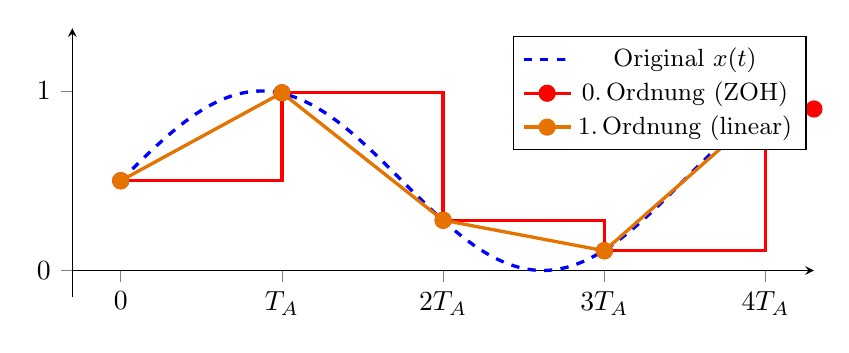
\begin{tikzpicture}
\begin{axis}[
    width=11cm, height=5cm,
    xmin=-0.3, xmax=4.3,
    ymin=-0.15, ymax=1.35,
    axis x line=middle,
    axis y line=left,
    xtick={0,1,2,3,4},
    xticklabels={$0$, $T_A$, $2T_A$, $3T_A$, $4T_A$},
    ytick={0,1},
    tick align=outside,
    legend style={at={(0.99,0.97)}, anchor=north east, font=\small},
    every axis plot/.append style={line width=1.2pt},
]
\addplot[blue, dashed, smooth, domain=0:4.2, samples=200] {0.5*sin(deg(x*1.8)) + 0.5};
\addlegendentry{Original $x(t)$}
\addplot[red, const plot, mark=*, mark size=2.5pt, mark options={fill=red}]
    coordinates {(0,0.50) (1,0.99) (2,0.28) (3,0.11) (4,0.90) (4.3,0.90)};
\addlegendentry{0.\,Ordnung (ZOH)}
\addplot[orange!90!black, sharp plot, mark=*, mark size=2.5pt,
         mark options={fill=orange!90!black}]
    coordinates {(0,0.50) (1,0.99) (2,0.28) (3,0.11) (4,0.90)};
\addlegendentry{1.\,Ordnung (linear)}
\end{axis}
\end{tikzpicture}
\caption{Interpolationsvergleich: Original (blau, gestrichelt), Zero-Order Hold (rot) und lineare
Interpolation (orange) anhand identischer Abtastwerte.}
\end{figure}

\subsubsection*{Die \texorpdfstring{$\operatorname{si}$}{si}-Funktion}

Die $\operatorname{si}$-Funktion (normierter Sinc) ist definiert als:

$$
\operatorname{si}(x) = \frac{\sin(\pi x)}{\pi x} \quad (x \neq 0),
\qquad \operatorname{si}(0) = 1
$$

Entscheidend ist die \textbf{Interpolationseigenschaft}: An ganzzahligen Argumenten gilt:

$$
\operatorname{si}(n) =
\begin{cases}
    1 & n = 0 \\
    0 & n \in \mathbb{Z},\; n \neq 0
\end{cases}
$$

Damit ist jede Basisfunktion $g_k(n \cdot T_A) = \operatorname{si}(n - k)$ genau an ihrem
eigenen Abtastzeitpunkt gleich $1$ und an allen anderen gleich $0$ – die Abtastwerte stören
sich gegenseitig nicht. Die vollständige Rekonstruktionsformel lautet:

$$
x(t) = \sum_{k=-\infty}^{\infty} x[k] \cdot \operatorname{si}\!\left(\frac{t - k T_A}{T_A}\right)
$$

\begin{figure}[H]
\centering
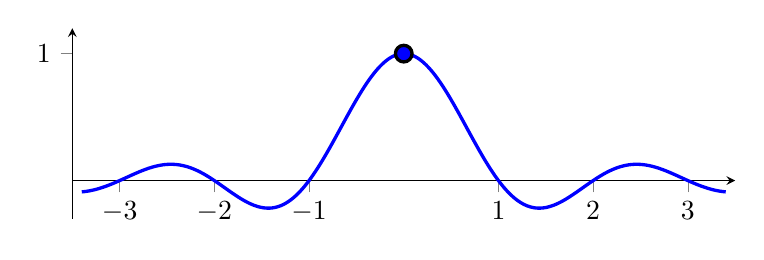
\begin{tikzpicture}
\begin{axis}[
    width=10cm, height=4cm,
    xmin=-3.5, xmax=3.5,
    ymin=-0.30, ymax=1.2,
    axis x line=middle,
    axis y line=left,
    xtick={-3,-2,-1,1,2,3},
    xticklabels={$-3$, $-2$, $-1$, $1$, $2$, $3$},
    ytick={1},
    yticklabels={$1$},
    tick align=outside,
    every axis plot/.append style={line width=1.2pt},
]
\addplot[blue, smooth, domain=-3.4:-0.03, samples=150] {sin(deg(pi*x))/(pi*x)};
\addplot[blue, smooth, domain= 0.03: 3.4, samples=150] {sin(deg(pi*x))/(pi*x)};
\addplot[only marks, mark=*, mark size=3pt, mark options={fill=blue}] coordinates {(0,1)};
\end{axis}
\end{tikzpicture}
\caption{$\operatorname{si}$-Funktion: Maximum bei $(0,\,1)$, Nullstellen bei allen
ganzzahligen $x \neq 0$.}
\end{figure}

\textbf{Beispiel Aufgabe}

Substituion üben:

Korrelation mit einem cos signal und einem rechtecksignal, wo substituiert werden muss.
Höllisch schwierig.

$$
\begin{array}{rl}
x_1(t) = & B \cdot rect(\frac{t+\frac{3}{2}T}{5T}) \\
x_2(t) = & \pi \cdot cos(\frac{5 \pi t}{T}) \\
=>  & \Phi_{x_1x_2}(\tau)
\end{array}
$$

Die Lösung ist:
$$
- \frac{2}{5} BT \cdot cos(\frac{5 \pi \tau}{T})
$$

Additionstheorem vollständig erlernen.

$$
sin(a-b) + sin(a+b) = 2 \cdot sin(a) \cdot cos(b)
$$

$$
\begin{array}{rl}
    sin(t+n \cdot 2 \pi) = & sin(t) \\
    sin(t) = & -sin(t)
\end{array}
$$

% ================================================================
%   Vorrechenaufgabe 4 – Ergänzung: Teil d) und e)
% ================================================================

\subsection*{Vorrechenaufgabe 4 – Ergänzung (Teil d und e)}

Die Teile a)–c) (Abtastung, Midrise-Kennlinie, Quantisierung) sowie f)–g)
(Interpolation) sind in den obigen Abschnitten bereits ausgearbeitet. Es fehlen
noch der Quantisierungsfehler (Teil~d) und die entstehende Datenmenge (Teil~e).

\subsubsection*{d) Quantisierungsfehler}

\begin{beispiel}[Quantisierungsfehler der abgetasteten und quantisierten Folge]

\textbf{Gegeben:} Die Abtastwerte $x[n]$ und die zugehörigen quantisierten Werte
$\hat{x}[n]$ aus Teil~c) (Midrise, $N = 4$, $\Delta x = 0{,}2$,
Rekonstruktionsniveaus $\{-0{,}3;\,-0{,}1;\,0{,}1;\,0{,}3\}$).

\textbf{Gesucht:} Der Quantisierungsfehler $e[n] = x[n] - \hat{x}[n]$ und der
Nachweis der Fehlerschranke.

\textbf{Formel} (Quantisierungsfehler und Fehlerschranke,
Abschnitt~\ref{sec:quantisierungsfehler}):

$$
e[n] = x[n] - \hat{x}[n], \qquad |e[n]| \leq \frac{\Delta x}{2}
$$

\textbf{Rechnung:}

Mit $\Delta x = 0{,}2$ beträgt die Fehlerschranke $\tfrac{\Delta x}{2} = 0{,}1$.
Differenzbildung für jeden Abtastwert:

\begin{center}
\begin{tabular}{c|cccccccccc}
\toprule
$n$ & 0 & 1 & 2 & 3 & 4 & 5 & 6 & 7 & 8 & 9 \\
\midrule
$x[n]$        & $0{,}38$ & $0{,}22$ & $-0{,}05$ & $-0{,}31$ & $-0{,}39$ & $-0{,}17$ & $0{,}08$ & $0{,}28$ & $0{,}39$ & $0{,}15$ \\
$\hat{x}[n]$  & $0{,}3$  & $0{,}3$  & $-0{,}1$  & $-0{,}3$  & $-0{,}3$  & $-0{,}1$  & $0{,}1$  & $0{,}3$  & $0{,}3$  & $0{,}1$ \\
$e[n]$        & $0{,}08$ & $-0{,}08$& $0{,}05$  & $-0{,}01$ & $-0{,}09$ & $-0{,}07$ & $-0{,}02$& $-0{,}02$& $0{,}09$ & $0{,}05$ \\
\bottomrule
\end{tabular}
\end{center}

\textbf{Lösung:}

$$
\boxed{\;|e[n]| \leq \frac{\Delta x}{2} = 0{,}1 \quad \text{für alle } n\;}
$$

Der Betrag des Quantisierungsfehlers überschreitet nie die halbe Stufenhöhe.

\begin{figure}[H]
\centering
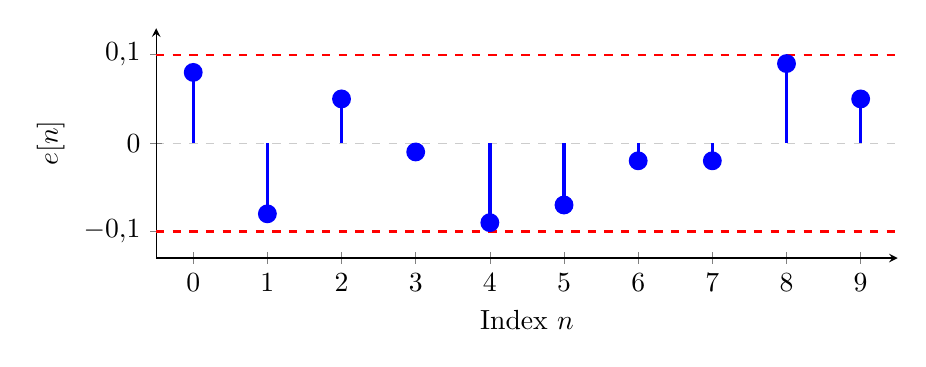
\begin{tikzpicture}
\begin{axis}[
    width=11cm, height=4.5cm,
    xlabel={Index $n$},
    ylabel={$e[n]$},
    xmin=-0.5, xmax=9.5,
    ymin=-0.13, ymax=0.13,
    axis lines=left,
    xtick={0,1,...,9},
    ytick={-0.1,0,0.1},
    yticklabels={$-0{,}1$, $0$, $0{,}1$},
    ymajorgrids=true,
    grid style={dashed, gray!40},
    every axis plot/.append style={line width=1.2pt},
]
% Fehlerschranken
\addplot[red, dashed, line width=0.8pt, domain=-0.5:9.5] {0.1};
\addplot[red, dashed, line width=0.8pt, domain=-0.5:9.5] {-0.1};
\addplot[blue, ycomb, mark=*, mark size=2.8pt, mark options={fill=blue}]
    coordinates {
        (0, 0.08) (1, -0.08) (2, 0.05) (3, -0.01) (4, -0.09)
        (5, -0.07) (6, -0.02) (7, -0.02) (8, 0.09) (9, 0.05)
    };
\end{axis}
\end{tikzpicture}
\caption{Quantisierungsfehler $e[n] = x[n] - \hat{x}[n]$. Alle Werte liegen
innerhalb der Schranken $\pm\Delta x/2 = \pm 0{,}1$ (rot gestrichelt).}
\end{figure}

\end{beispiel}

\subsubsection*{e) Datenmenge}

\begin{beispiel}[Datenrate bei binärer Codierung der Quantisierungsniveaus]

\textbf{Gegeben:} Abtastfrequenz $f_A = 10\,\text{kHz}$, Quantisierung mit
$N = 4$ Stufen. Die Niveaus werden natürlichen binären Zahlen zugeordnet.

\textbf{Gesucht:} Die entstehende Datenrate (Datenmenge pro Zeit).

\textbf{Formel} (Wortbreite und Datenrate, Abschnitt~\ref{sec:codierung-binaer}):

$$
w = \log_2 N, \qquad R = f_A \cdot w
$$

\textbf{Rechnung:}

Für $N = 4$ Quantisierungsniveaus werden

$$
w = \log_2 4 = 2 \ \text{Bit}
$$

pro Abtastwert benötigt. Bei $f_A = 10\,\text{kHz} = 10\,000\ \text{Abtastwerte/s}$
folgt

$$
R = f_A \cdot w = 10\,000\,\text{s}^{-1} \cdot 2\,\text{Bit}
  = 20\,000\ \frac{\text{Bit}}{\text{s}}.
$$

\textbf{Lösung:}

$$
\boxed{\;w = 2\ \text{Bit}, \qquad R = 20\,000\ \frac{\text{Bit}}{\text{s}}
= 20\ \frac{\text{kbit}}{\text{s}}\;}
$$

Jeder Abtastwert benötigt $2$~Bit; pro Sekunde entstehen somit $20$~kbit.

\end{beispiel}

% ================================================================
%   Aufgabe 4.1 – Datenrate, Datenmenge (Audio-CD)
% ================================================================

\subsection*{Aufgabe 4.1 – Datenrate und Datenmenge (Audio-CD)}

Auf einer Audio-CD wird zweikanalig (Stereo) gespeichert. Jeder der beiden Kanäle
wird mit $f_A = 44{,}1\,\text{kHz}$ abgetastet und mit $w = 16$~Bit quantisiert.

\subsubsection*{a) Datenrate des Stereosignals}

\begin{beispiel}[Datenrate eines Stereosignals]

\textbf{Gegeben:} $K = 2$ Kanäle, $f_A = 44{,}1\,\text{kHz}$, $w = 16$~Bit.

\textbf{Gesucht:} Die Datenrate $R$ in kbit/s.

\textbf{Formel} (Datenrate, Abschnitt~\ref{sec:codierung-binaer}):

$$
R = K \cdot f_A \cdot w
$$

\textbf{Rechnung:}

$$
R = 2 \cdot 44\,100\,\text{s}^{-1} \cdot 16\,\text{Bit}
  = 1\,411\,200\ \frac{\text{Bit}}{\text{s}}.
$$

\textbf{Lösung:}

$$
\boxed{\;R = 1\,411\,200\ \frac{\text{Bit}}{\text{s}}
= 1411{,}2\ \frac{\text{kbit}}{\text{s}} \approx 1{,}41\ \frac{\text{Mbit}}{\text{s}}\;}
$$

\end{beispiel}

\subsubsection*{b) Maximal reproduzierbare Signalfrequenz}

\begin{beispiel}[Maximale Signalfrequenz nach dem Abtasttheorem]

\textbf{Gegeben:} $f_A = 44{,}1\,\text{kHz}$ (Quantisierung vernachlässigt).

\textbf{Gesucht:} Die maximale fehlerfrei reproduzierbare Signalfrequenz
$f_{\max}$.

\textbf{Formel} (Abtasttheorem, Abschnitt~\ref{sec:abtasttheorem}):

$$
f_A > 2\, f_{\max} \quad\Longrightarrow\quad f_{\max} = \frac{f_A}{2}
$$

\textbf{Rechnung:}

$$
f_{\max} = \frac{44{,}1\,\text{kHz}}{2} = 22{,}05\,\text{kHz}.
$$

\textbf{Lösung:}

$$
\boxed{\;f_{\max} = \frac{f_A}{2} = 22{,}05\,\text{kHz}\;}
$$

Dies deckt den gesamten für den Menschen hörbaren Bereich (bis ca.\ $20\,\text{kHz}$) ab.

\end{beispiel}

\subsubsection*{c) Datenmenge der Goldberg-Variationen}

\begin{beispiel}[Datenmenge zweier Aufnahmen unterschiedlicher Dauer]

\textbf{Gegeben:} Datenrate $R = 1\,411\,200\ \text{Bit/s}$ (aus Teil~a).
Dauer der Aufnahme von 1955: $t_1 = 38\,\text{min}\,25\,\text{s}$; von 1982:
$t_2 = 51\,\text{min}\,20\,\text{s}$.

\textbf{Gesucht:} Die zu speichernde Datenmenge $D$ beider Aufnahmen.

\textbf{Formel} (Datenmenge aus Datenrate und Dauer):

$$
D = R \cdot t
$$

\textbf{Rechnung:}

Umrechnung der Spielzeiten in Sekunden:

$$
t_1 = 38 \cdot 60 + 25 = 2305\,\text{s}, \qquad
t_2 = 51 \cdot 60 + 20 = 3080\,\text{s}.
$$

Aufnahme 1955:

$$
D_1 = 1\,411\,200\ \tfrac{\text{Bit}}{\text{s}} \cdot 2305\,\text{s}
    = 3\,252\,816\,000\ \text{Bit}
    = \frac{D_1}{8} = 406\,602\,000\ \text{Byte} \approx 406{,}6\ \text{MB}.
$$

Aufnahme 1982:

$$
D_2 = 1\,411\,200\ \tfrac{\text{Bit}}{\text{s}} \cdot 3080\,\text{s}
    = 4\,346\,496\,000\ \text{Bit}
    = 543\,312\,000\ \text{Byte} \approx 543{,}3\ \text{MB}.
$$

\textbf{Lösung:}

$$
\boxed{\;D_1 \approx 406{,}6\ \text{MB} \; (2305\,\text{s}), \qquad
D_2 \approx 543{,}3\ \text{MB} \; (3080\,\text{s})\;}
$$

Die langsamere Aufnahme von 1982 benötigt entsprechend ihrer längeren Spieldauer
mehr Speicher (Umrechnung mit $1\,\text{MB} = 10^6\,\text{Byte}$; mit
$1\,\text{MiB} = 2^{20}\,\text{Byte}$ ergäben sich $387{,}8$ bzw.\ $518{,}1$~MiB).

\end{beispiel}

% ================================================================
%   Aufgabe 4.2 – Quantisierungsfehler
% ================================================================

\subsection*{Aufgabe 4.2 – Quantisierungsfehler}

Ein zeitdiskretes Signal mit Wertebereich $[-1,\,1]$ (Spannweite
$x_{\max} - x_{\min} = 2$) soll so quantisiert werden, dass die Leistung des
Quantisierungsfehlers $P_e = 0{,}01$ beträgt.

\subsubsection*{a) Erforderliche Stufenhöhe}

\begin{beispiel}[Stufenhöhe aus vorgegebener Fehlerleistung]

\textbf{Gegeben:} Fehlerleistung $P_e = 0{,}01$.

\textbf{Gesucht:} Die maximal zulässige Stufenhöhe $\Delta x$.

\textbf{Formel} (Leistung des Quantisierungsfehlers,
Abschnitt~\ref{sec:quantisierungsfehler}):

$$
P_e = \frac{\Delta x^2}{12}
$$

\textbf{Rechnung:}

Nach $\Delta x$ auflösen:

$$
\Delta x = \sqrt{12\, P_e} = \sqrt{12 \cdot 0{,}01} = \sqrt{0{,}12}.
$$

\textbf{Lösung:}

$$
\boxed{\;\Delta x = \sqrt{0{,}12} \approx 0{,}346\;}
$$

Um $P_e = 0{,}01$ nicht zu überschreiten, darf die Stufenhöhe höchstens
$\Delta x \approx 0{,}346$ betragen.

\end{beispiel}

\subsubsection*{b) Mindestanzahl der Bits}

\begin{beispiel}[Wortbreite bei binärer Codierung]

\textbf{Gegeben:} Spannweite $x_{\max} - x_{\min} = 2$, maximale Stufenhöhe
$\Delta x \approx 0{,}346$ (aus Teil~a).

\textbf{Gesucht:} Die mindestens erforderliche Wortbreite $w$ (Bit pro
Abtastwert).

\textbf{Formel} (Stufenzahl und Wortbreite,
Abschnitte~\ref{sec:quantisierung} und~\ref{sec:codierung-binaer}):

$$
N = \frac{x_{\max} - x_{\min}}{\Delta x}, \qquad w = \left\lceil \log_2 N \right\rceil
$$

\textbf{Rechnung:}

Erforderliche Stufenzahl:

$$
N = \frac{2}{\sqrt{0{,}12}} = \frac{2}{0{,}346} \approx 5{,}77
\quad\Longrightarrow\quad N \geq 6.
$$

Da nur ganze Bit vergeben werden, ist auf die nächste Zweierpotenz aufzurunden:

$$
w = \left\lceil \log_2 6 \right\rceil = \left\lceil 2{,}585 \right\rceil = 3\,\text{Bit}
\qquad (2^3 = 8 \geq 6).
$$

Kontrolle: Mit $w = 3$~Bit ($8$~Stufen) wird
$\Delta x = \tfrac{2}{8} = 0{,}25$ und

$$
P_e = \frac{0{,}25^2}{12} \approx 0{,}0052 \leq 0{,}01. \quad\checkmark
$$

Mit nur $w = 2$~Bit ($4$~Stufen) wäre $\Delta x = 0{,}5$ und
$P_e = \tfrac{0{,}25}{12} \approx 0{,}0208 > 0{,}01$ -- unzureichend.

\textbf{Lösung:}

$$
\boxed{\;w = 3\ \text{Bit pro Abtastwert}\;}
$$

\end{beispiel}

% ================================================================
%   Aufgabe 4.3 – Datenmenge und Übertragungsdauer
% ================================================================

\subsection*{Aufgabe 4.3 – Datenmenge und Übertragungsdauer}

\subsubsection*{Datenmenge eines Bildes}

\begin{beispiel}[Datenmenge eines Vollbildes]

\textbf{Gegeben:} Bild mit $1920 \times 1080$ Bildpunkten, jeder Bildpunkt mit
$24$~Bit dargestellt.

\textbf{Gesucht:} Die Datenmenge $D$ des Bildes.

\textbf{Formel} (Datenmenge, Abschnitt~\ref{sec:codierung-binaer}):

$$
D = N_{\text{Pixel}} \cdot w = (n_x \cdot n_y) \cdot w
$$

\textbf{Rechnung:}

$$
D = 1920 \cdot 1080 \cdot 24\,\text{Bit}
  = 2\,073\,600 \cdot 24\,\text{Bit}
  = 49\,766\,400\ \text{Bit}.
$$

In Byte:

$$
D = \frac{49\,766\,400}{8}\ \text{Byte} = 6\,220\,800\ \text{Byte}
  \approx 6{,}22\ \text{MB}.
$$

\textbf{Lösung:}

$$
\boxed{\;D = 49\,766\,400\ \text{Bit} \approx 6{,}22\ \text{MB}\;}
$$

\end{beispiel}

\subsubsection*{a)–d) Übertragungsdauer über verschiedene Verbindungen}

\begin{beispiel}[Übertragungsdauer aus Datenmenge und Übertragungsrate]

\textbf{Gegeben:} Datenmenge $D = 49\,766\,400\ \text{Bit}$; Übertragungsraten
EDGE $R_a = 236{,}8\,\text{kbit/s}$, UMTS $R_b = 7{,}2\,\text{Mbit/s}$, LTE
$R_c = 150\,\text{Mbit/s}$, VDSL $R_d = 210\,\text{Mbit/s}$.

\textbf{Gesucht:} Die jeweilige Übertragungsdauer $t = D / R$.

\textbf{Formel} (Übertragungsdauer):

$$
t = \frac{D}{R}
$$

\textbf{Rechnung:}

$$
t_a = \frac{49\,766\,400\,\text{Bit}}{236\,800\ \text{Bit/s}} \approx 210{,}2\,\text{s}
    \approx 3\,\text{min}\,30\,\text{s} \quad (\text{EDGE})
$$

$$
t_b = \frac{49\,766\,400\,\text{Bit}}{7\,200\,000\ \text{Bit/s}} \approx 6{,}91\,\text{s}
    \quad (\text{UMTS})
$$

$$
t_c = \frac{49\,766\,400\,\text{Bit}}{150\,000\,000\ \text{Bit/s}} \approx 0{,}332\,\text{s}
    \quad (\text{LTE})
$$

$$
t_d = \frac{49\,766\,400\,\text{Bit}}{210\,000\,000\ \text{Bit/s}} \approx 0{,}237\,\text{s}
    \quad (\text{VDSL})
$$

\textbf{Lösung:}

$$
\boxed{\;t_a \approx 210{,}2\,\text{s}, \quad t_b \approx 6{,}91\,\text{s}, \quad
t_c \approx 0{,}332\,\text{s}, \quad t_d \approx 0{,}237\,\text{s}\;}
$$

Mit steigender Übertragungsrate sinkt die Übertragungsdauer entsprechend: von über
drei Minuten (EDGE) auf einen Bruchteil einer Sekunde (VDSL).

\end{beispiel}

% ================================================================
%   Aufgabe 4.4 – Adaptives Scheinwerferlicht
% ================================================================

\subsection*{Aufgabe 4.4 – Adaptives Scheinwerferlicht}

Die Scheinwerferausrichtung wird über den Lenkradeinschlagwinkel gesteuert. Das
Lenkrad kann maximal um $[-360^\circ,\, 360^\circ]$ eingeschlagen werden. Bei
Maximalausschlag dürfen die Scheinwerfer für Geschwindigkeiten unter
$30\,\tfrac{\text{km}}{\text{h}}$ um $20^\circ$, für Geschwindigkeiten über
$30\,\tfrac{\text{km}}{\text{h}}$ um $10^\circ$ verstellt werden. Die Verstellung
erfolgt in $5^\circ$-Schritten.

\subsubsection*{a) Benötigte Sensoren und Informationen}

\begin{beispiel}[Sensorik des adaptiven Scheinwerfers]

\textbf{Gegeben:} Steuerung der Scheinwerfer nach Lenkradwinkel und
geschwindigkeitsabhängiger Fallunterscheidung.

\textbf{Gesucht:} Anzahl und Aufgabe der benötigten Sensoren.

\textbf{Lösung:}

Es werden \textbf{zwei} Sensoren benötigt:

\begin{itemize}
  \item \textbf{Lenkwinkelsensor:} misst den Lenkradeinschlagwinkel im Bereich
        $[-360^\circ,\, 360^\circ]$. Er liefert die Richtungsinformation für die
        Scheinwerferverstellung.
  \item \textbf{Geschwindigkeitssensor:} misst die Fahrgeschwindigkeit. Benötigt
        wird nur die Unterscheidung, ob $v < 30\,\tfrac{\text{km}}{\text{h}}$
        (Fall~1, $\pm 20^\circ$) oder $v > 30\,\tfrac{\text{km}}{\text{h}}$
        (Fall~2, $\pm 10^\circ$) vorliegt.
\end{itemize}

$$
\boxed{\;\text{2 Sensoren: Lenkwinkel (Richtung) und Geschwindigkeit (Fallwahl)}\;}
$$

\end{beispiel}

\subsubsection*{b) Quantisierungskennlinien und Bitbedarf}

\begin{beispiel}[Kennlinien und Wortbreite der Sensoren]

\textbf{Gegeben:} Lenkwinkelbereich $[-360^\circ, 360^\circ]$ (Spannweite
$720^\circ$); Scheinwerfer in $5^\circ$-Schritten, maximal $\pm 20^\circ$
(Fall~1) bzw.\ $\pm 10^\circ$ (Fall~2).

\textbf{Gesucht:} Die Quantisierungskennlinien sowie die Wortbreite $w$ für die
Codierung.

\textbf{Formel} (Stufenzahl und Wortbreite,
Abschnitte~\ref{sec:quantisierungskennlinie} und~\ref{sec:codierung-binaer}):

$$
w = \left\lceil \log_2 N \right\rceil
$$

\textbf{Rechnung:}

\emph{Fall 1} ($v < 30\,\tfrac{\text{km}}{\text{h}}$): Scheinwerferpositionen
$\{-20, -15, -10, -5, 0, 5, 10, 15, 20\}^\circ$, also $N_1 = 9$ Stufen. Der
gesamte Lenkbereich $720^\circ$ wird auf $9$~Stufen abgebildet (Midtread, damit
Geradeausfahrt $0^\circ \to 0^\circ$), Stufenbreite $720^\circ/9 = 80^\circ$.

\emph{Fall 2} ($v > 30\,\tfrac{\text{km}}{\text{h}}$): Scheinwerferpositionen
$\{-10, -5, 0, 5, 10\}^\circ$, also $N_2 = 5$ Stufen, Stufenbreite
$720^\circ/5 = 144^\circ$.

Der Lenkwinkelsensor muss den anspruchsvolleren Fall~1 auflösen:

$$
w_{\text{Lenk}} = \left\lceil \log_2 9 \right\rceil = 4\,\text{Bit}
\qquad (2^4 = 16 \geq 9).
$$

Der Geschwindigkeitssensor muss nur zwei Zustände unterscheiden:

$$
w_{\text{Geschw}} = \left\lceil \log_2 2 \right\rceil = 1\,\text{Bit}.
$$

\textbf{Lösung:}

$$
\boxed{\;w_{\text{Lenk}} = 4\ \text{Bit}, \quad w_{\text{Geschw}} = 1\ \text{Bit},
\quad w_{\text{ges}} = 5\ \text{Bit}\;}
$$

\begin{figure}[H]
\centering
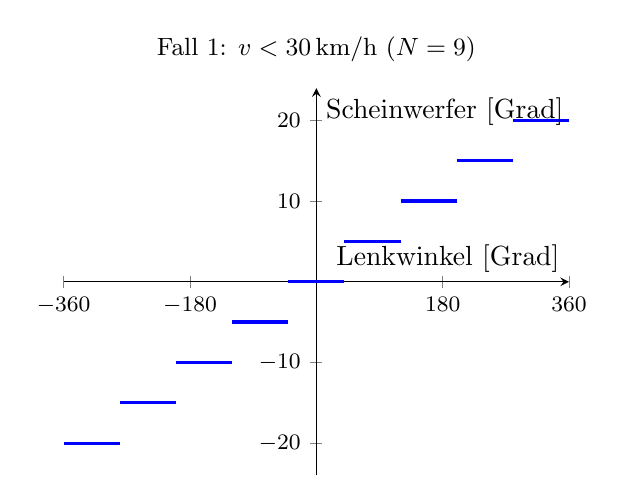
\begin{tikzpicture}
\begin{axis}[
    width=8cm, height=6.5cm,
    xlabel={Lenkwinkel [Grad]},
    ylabel={Scheinwerfer [Grad]},
    title={Fall 1: $v < 30\,$km/h ($N=9$)},
    title style={font=\small},
    xmin=-360, xmax=360, ymin=-24, ymax=24,
    axis lines=center,
    xtick={-360,-180,180,360},
    ytick={-20,-10,10,20},
    tick label style={font=\footnotesize},
    every axis plot/.append style={line width=1.2pt},
]
\addplot[blue] coordinates {(-360,-20) (-280,-20)};
\addplot[blue] coordinates {(-280,-15) (-200,-15)};
\addplot[blue] coordinates {(-200,-10) (-120,-10)};
\addplot[blue] coordinates {(-120,-5) (-40,-5)};
\addplot[blue] coordinates {(-40,0) (40,0)};
\addplot[blue] coordinates {(40,5) (120,5)};
\addplot[blue] coordinates {(120,10) (200,10)};
\addplot[blue] coordinates {(200,15) (280,15)};
\addplot[blue] coordinates {(280,20) (360,20)};
\end{axis}
\end{tikzpicture}
\hfill
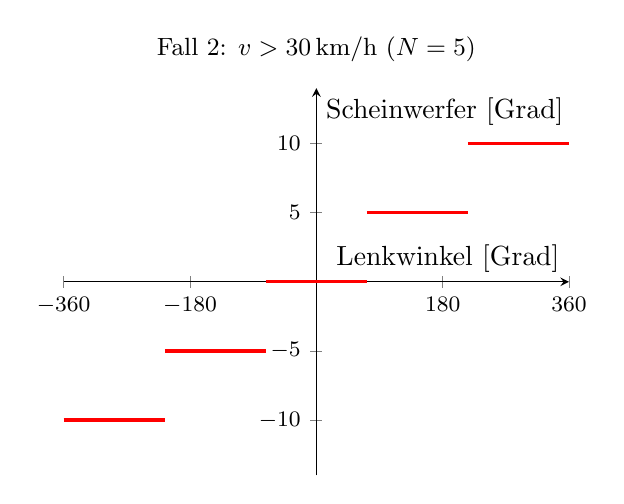
\begin{tikzpicture}
\begin{axis}[
    width=8cm, height=6.5cm,
    xlabel={Lenkwinkel [Grad]},
    ylabel={Scheinwerfer [Grad]},
    title={Fall 2: $v > 30\,$km/h ($N=5$)},
    title style={font=\small},
    xmin=-360, xmax=360, ymin=-14, ymax=14,
    axis lines=center,
    xtick={-360,-180,180,360},
    ytick={-10,-5,5,10},
    tick label style={font=\footnotesize},
    every axis plot/.append style={line width=1.2pt},
]
\addplot[red] coordinates {(-360,-10) (-216,-10)};
\addplot[red] coordinates {(-216,-5) (-72,-5)};
\addplot[red] coordinates {(-72,0) (72,0)};
\addplot[red] coordinates {(72,5) (216,5)};
\addplot[red] coordinates {(216,10) (360,10)};
\end{axis}
\end{tikzpicture}
\caption{Quantisierungskennlinien (Midtread) des Lenkwinkelsensors: links Fall~1
($9$~Stufen, $\pm 20^\circ$), rechts Fall~2 ($5$~Stufen, $\pm 10^\circ$).}
\end{figure}

\end{beispiel}

\subsubsection*{c) Mögliches Problem und Abhilfe}

\begin{beispiel}[Unterabtastung und Flackern]

\textbf{Gegeben:} Zeitdiskrete Abtastung des schnell veränderlichen
Lenkwinkelverlaufs.

\textbf{Gesucht:} Ein Realisierungsproblem und geeignete Gegenmaßnahmen.

\textbf{Lösung:}

Wird die Abtastrate zu niedrig gewählt (z.\,B.\ $1\,\text{Hz}$), so verletzt sie
für schnelle Lenkbewegungen das Abtasttheorem
(Abschnitt~\ref{sec:abtasttheorem}). Es kommt zu \textbf{Unterabtastung
(Aliasing)}: Die Scheinwerfer folgen dem Lenkeinschlag nur verzögert oder falsch,
weil zwischen zwei Abtastzeitpunkten große Winkeländerungen unbemerkt bleiben.
Zusätzlich kann der quantisierte Wert an einer Stufengrenze zwischen zwei Niveaus
\textbf{hin- und herspringen (Flackern)}.

$$
\boxed{\;\text{Abhilfe: höhere Abtastrate (Abtasttheorem) + Hysterese gegen Flackern}\;}
$$

Eine höhere Abtastfrequenz stellt sicher, dass die Scheinwerfer der Lenkbewegung
zeitgerecht folgen; eine Hysterese an den Stufengrenzen unterdrückt das Flackern.

\end{beispiel}

\subsubsection*{d) Ausrichtung bei 1 Hz Abtastung mit Beschleunigung}

\begin{beispiel}[Abtastung des Lenkverlaufs und Scheinwerferausrichtung]

\textbf{Gegeben:} Lenkwinkelverlauf gemäß Abbildung, Abtastrate $f_A = 1\,\text{Hz}$
(Abtastung bei $t = 0, 1, \ldots, 12\,\text{s}$). Das Fahrzeug fährt bis
$t = 6\,\text{s}$ mit $25\,\tfrac{\text{km}}{\text{h}}$ (Fall~1, $\pm 20^\circ$)
und beschleunigt danach auf $35\,\tfrac{\text{km}}{\text{h}}$ (Fall~2,
$\pm 10^\circ$).

\textbf{Gesucht:} Die quantisierte Scheinwerferausrichtung zu jedem
Abtastzeitpunkt.

\textbf{Formel} (lineare Zuordnung Lenkwinkel $\varphi$ $\to$ Scheinwerferwinkel,
anschließend Quantisierung in $5^\circ$-Schritten,
Abschnitt~\ref{sec:quantisierungskennlinie}):

$$
\text{Fall 1: } \hat{s} = \operatorname{round}_{5^\circ}\!\left(\frac{\varphi}{360^\circ}\cdot 20^\circ\right),
\qquad
\text{Fall 2: } \hat{s} = \operatorname{round}_{5^\circ}\!\left(\frac{\varphi}{360^\circ}\cdot 10^\circ\right)
$$

\textbf{Rechnung:}

Zunächst werden die Lenkwinkel $\varphi(t)$ zu den ganzzahligen Sekunden aus dem
Diagramm abgelesen (Werte gerundet). Für $t < 6\,\text{s}$ gilt Fall~1
(Skalierung $\varphi/18$), für $t \geq 6\,\text{s}$ Fall~2 (Skalierung
$\varphi/36$); anschließend wird auf das nächste Vielfache von $5^\circ$
gerundet und auf $\pm 20^\circ$ bzw.\ $\pm 10^\circ$ begrenzt:

\begin{center}
\begin{tabular}{c|c|c|c|c|c}
\toprule
$t$/s & $\varphi$/Grad & $v$/(km/h) & Fall & ideal/Grad & $\hat{s}$/Grad \\
\midrule
0  & $0$    & 25 & 1 & $0{,}0$   & $0$   \\
1  & $-80$  & 25 & 1 & $-4{,}4$  & $-5$  \\
2  & $+100$ & 25 & 1 & $+5{,}6$  & $+5$  \\
3  & $+190$ & 25 & 1 & $+10{,}6$ & $+10$ \\
4  & $-350$ & 25 & 1 & $-19{,}4$ & $-20$ \\
5  & $+30$  & 25 & 1 & $+1{,}7$  & $0$   \\
\midrule
6  & $+150$ & 35 & 2 & $+4{,}2$  & $+5$  \\
7  & $-40$  & 35 & 2 & $-1{,}1$  & $0$   \\
8  & $+120$ & 35 & 2 & $+3{,}3$  & $+5$  \\
9  & $+150$ & 35 & 2 & $+4{,}2$  & $+5$  \\
10 & $-110$ & 35 & 2 & $-3{,}1$  & $-5$  \\
11 & $-40$  & 35 & 2 & $-1{,}1$  & $0$   \\
12 & $+20$  & 35 & 2 & $+0{,}6$  & $0$   \\
\bottomrule
\end{tabular}
\end{center}

\textbf{Lösung:}

$$
\boxed{\;
\begin{array}{l}
\hat{s}(0\ldots5) = (0,\, -5,\, +5,\, +10,\, -20,\, 0)^\circ \quad (\text{Fall 1}) \\[4pt]
\hat{s}(6\ldots12) = (+5,\, 0,\, +5,\, +5,\, -5,\, 0,\, 0)^\circ \quad (\text{Fall 2})
\end{array}\;}
$$

Ab $t = 6\,\text{s}$ (Beschleunigung über $30\,\tfrac{\text{km}}{\text{h}}$) wird
der zulässige Verstellbereich auf $\pm 10^\circ$ halbiert; identische
Lenkwinkel führen dann zu kleineren Scheinwerferauslenkungen. Wegen der niedrigen
Abtastrate von $1\,\text{Hz}$ werden die schnellen Ausschläge des Lenkverlaufs nur
grob erfasst (vgl.\ Teil~c).

\end{beispiel}
